\lab{Algorithms}{An Introduction to Parallel Programming using MPI}{Introduction to Parallel Programming}
\objective{Learn the basics of parallel computing on distributed memory machines using MPI for Python}
\label{lab:MPI_Intro}

\section*{Why Parallel Computing?}
Over the past few decades, vast increases in computational power have come
through increased single processor performance, which have almost wholly been
driven by smaller transistors. However, these faster transistors generate more
heat, which destabilizes circuits. The so- called ``heat wall'' refers to the
physical limits of single processors to become faster because of the growing
inability to sufficiently dissipate heat.

Parallel computing was invented to circumvent this physical limitation. It
began, as with most things, in many different systems and styles. Some systems
had shared memory between many processors and some systems had a separate
program for each processor while others ran all the processors off the same base
program.

Today, the most commonly used method for high performance computing is a single-
program, multiple-data system with message passing. Essentially, this means that
supercomputers are made up of many, many normal computers, each with their own
memory. These normal computers are all running the same program and are able to
communicate with each other. Although they all run the same program file, each
process takes a different execution path through the code, as a result of the
interactions that message passing makes possible.

Note that the commands being executed by two different processes are going to be
different. Thus, we could actually write two separate computer programs in
different files to accomplish this. However, the most common method today has
become to write both processes in a single program, using conditionals and
techniques from the Message Passing Interface to control which lines of code get
executed by each process.

This is a very different architecture than ``normal'' computers, and it requires
a different kind of software. You can't take a traditional program and expect it
to magically run faster on a supercomputer; you must design new algorithms in
ways that take advantage of the unique advantages of parallel computing.

\section*{MPI: the Message Passing Interface}
At its most basic, the Message Passing Interface (MPI) provides functions for
sending and receiving messages between different processes. You can think of a
process as one of the many ``normal'' computers that make up a supercomputer.

MPI was developed out of the need for standardization of programming parallel
systems. It is different than other approaches in that MPI does not require
programs to be written in a particular language. Rather, MPI specifies a library
of functions--the syntax and semantics of message passing routines--that can be
called from other programming languages, such as Python and C. MPI provides a
very powerful and very general way of expressing parallelism. It can be thought
of as ``the assembly language of parallel computing,'' because of this
generality and the detail that it forces the programmer to deal
with\footnote{Parallel Programming with MPI, by Peter S. Pacheco, p. 7}. In
spite of this apparent drawback, MPI is still very important. It was the first
portable, universally available standard for programming parallel systems, and
it is the \emph{de facto} standard today. MPI makes it possible for programmers
to develop portable, parallel software libraries. Until recently, one of the
biggest problems in parallel computing was the lack of software. However,
parallel software is growing faster thanks in large part to this
standardization.

% \begin{problem}
% Most modern personal computers now have multicore processors. In
% order to take advantage of the extra available computational power, a single
% program must be specially designed. Programs that are designed for these
% multicore processors are also ``parallel'' programs, typically written using
% POSIX threads or OpenMP. MPI, on the other hand, is designed with a different
% kind of architecture in mind. How does the architecture of a system for which
% MPI is designed differ what POSIX threads or OpenMP is designed for? What is the
% difference between MPI and OpenMP or Pthreads?
% \label{prob:MPI_Intro:MPI_v_threads}
% \end{problem}
% TODO research this yourself and figure out whether multiple MPI processes can be run on a single computer

\section*{Why MPI for Python?}
In general, parallel programs are much more difficult and complex than
``normal'', serial programs. Python is an excellent language for algorithm
design and for solving problems that don't require maximum performance. This
makes Python great for prototyping and writing small or medium-sized parallel
programs. However, Python is not designed specifically for high performance
computing and its parallel capabilities are still somewhat underdeveloped, so in
practice it is better to write production code in fast, compiled languages, such
as C or Fortran.

We will use the Python library \texttt{mpi4py}. This package implements the
Message Passing Interface in a basic way that makes it relatively easy to port
your code to a faster language such as C for production code.

\section*{Introduction to MPI}
As tradition has it, we will start with a Hello World program.
\lstinputlisting[style=fromfile]{hello.py}
Save this program as \texttt{hello.py} and execute it from the command line as follows:
\begin{lstlisting}[style=ShellInput]
$ mpirun -n 3 python hello.py
\end{lstlisting}
\begin{info}
If the program fails to start, you may need to try the following syntax:
\begin{lstlisting}[style=ShellInput]
$ mpirun -n 3 python.exe hello.py
\end{lstlisting}
If you are on a Windows machine, you can also try using PowerShell instead of
Command Prompt if you still can't get it to work.
\end{info}
The program should output something like this:
\begin{lstlisting}[style=ShellOutput]
Hello world! I'm process number 2 out of 3.
Hello world! I'm process number 0 out of 3.
Hello world! I'm process number 1 out of 3.
\end{lstlisting}

Notice that when you try this on your own, the lines will not necessarily print
in order. The five processes will run autonomously, so their output could be
printed in any order.

\begin{warn}
Unless you are debugging, it is usually bad practice to perform I/O (e.g., call
\li{print}) from any process other than the root process (the \emph{root
process} is the process with rank 0)
\end{warn}

\section*{Execution}
How does this program work? When we execute
\begin{lstlisting}[style=ShellInput]
$ mpirun -n 3 python hello.py
\end{lstlisting}
a number of things happen:

First, the \texttt{mpirun} program is launched. This is the program which starts
MPI, a wrapper around whatever program you to pass into it. The ``-n 3'' option
specifies the desired number of processes. In this case, three processes are
initialized. The rest of this command, ``python hello.py'', is the command that
each process will run. Thus, each of the five processes will run a copy of
\texttt{hello.py} in its own execution environment, separate from the other two
processes. These three execution environments are identical except for one key
difference: Each process is assigned a different ``rank'' within the
\texttt{mpirun} program. Because of this, each process prints a different number
when it executes.

What are ranks and how do they work? When \texttt{mpirun} is first executed, it
creates a global communicator object. Each process can access can access this
object through the variable \li{MPI.COMM_WORLD} within the Python program. One
of the main purposes of this communicator is to keep track of each process's
``rank'', which is a unique identifier.

When each process executes the line \li{RANK = COMM.Get_rank()}, the process
queries the global communicator to figure out what the process's ``rank'' is.
Process ranks are essential to interprocess communication and coordination
because they are the only difference between each process's otherwise identical
execution environment.

After each process executes the line \li{RANK = COMM.Get_rank()}, each process's
local variable \li{RANK} will be different from each of the other two processes.
This gives us a way to distinguish between different processes while allowing us
to write the source code for the three processes in a single file.

\section*{MPI Communicators}
An MPI communicator object basically just represents a collection of processes.
Although processes can access communicators through the interface MPI provides,
communicators' data is stored within the execution environment of the
\texttt{mpirun} environment, not within the execution environments of the
individual processes.

Communicators allow processes to send and receive messages. In most of our
programs we will only deal with the \li{MPI.COMM_WORLD} communicator, which
contains all of the running processes.

\begin{figure}[htbp]
\centering
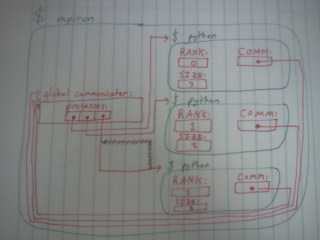
\includegraphics[width=.9\textwidth]{MPI_program_structure_placeholder.png}
\caption{A visualization of how MPI programs are structured. TODO get a better picture.}
\label{fig:MPI_program_structure}
\end{figure}

Figure~\ref{fig:MPI_program_structure} demonstrates how MPI programs are
structured. Each of the python processes execute independently from the others.
%TODO explain this better
%TODO Get better graphic

\begin{info}
In more advanced MPI programs, it is possible to create custom communicators
that group certain subsets of the processes together. This can be useful
(especially in supercomputers) because MPI can physically rearrange which
processes are assigned to which CPUs, thereby optimizing your program's speed by
making sure that the processes within each communicator can quickly communicate
with each other.

Note that a single process can be a member of many different communicators, and
that its rank will most likely be different in each communicator. However, since
our programs will just be using the global communicator \li{MPI.COMM_WORLD}, we
can think of ranks as being unique IDs assigned to each process.
\end{info}

\begin{problem}
Write a program \texttt{helloGoodbye.py} in which the the processes with an even
rank print ``Hello'' and process with an odd rank print ``Goodbye''.
Additionally, each process should print its rank and the total number of
processes currently running. This program should work for any number of
processes. For example, if you run this program with 6 processes, process 3
should print ``Goodbye from process 3 out of 6''.
\label{prob:MPI_Intro:helloGoodbye.py}
\end{problem}

\begin{problem}
This problem will teach you about \li{COMM.Abort()} and \li{COMM.Barrier()}.

Sometimes, a parallel algorithm can only run correctly if it has a certain
number of processes. Although you typically want to avoid writing these kinds of
programs, sometimes it is inconvenient or unavoidable. Write a program that runs
only if it has exactly 5 processes.

If there are not exactly 5 processes, the root process should print ``Error:
This program must run with exactly 5 processes.'' and call \li{COMM.Abort()},
which basically forces your program to stop immediately.

If there are exactly 5 processes, \emph{every} process should print
``Success!''. When a process calls \li{COMM.Barrier()}, it will freeze until
\emph{all} processes have called \li{COMM.Barrier()}. If you don't use this, it
is possible some process might execute \li{print \"Success\"} before process 0
has a chance to check whether there are exactly 5 processes.
\label{prob:MPI_Intro:AbortBarrier.py}
\end{problem}

\section*{Simple Message Passing}
With message passing, the processes in our programs can interact. Let us begin
by demonstrating a program designed for two processes. One will draw a random
number and then send it to the other. We will do this using the methods
\li{COMM.Send} and \li{COMM.Recv} (short for ``receive''):

\lstinputlisting[style=fromfile]{passValue.py}

To illustrate simple message passing, we have one process choose a random number
and then pass it to the other. Inside the receiving process, we have it print
out the value of the variable \li{receive_buffer} \emph{before} it calls
\li{Recv} to prove that it really is receiving the variable through the message
passing interface.

\begin{warn}
Due to the implementation of Python and mpi4py, you \emph{must} use a numpy
array to send and receive messages. When receiving a message, the receiving
array must be of the same size and data type as the array that was sent.
% TODO add more info here about WHY
\end{warn}

Here is the syntax for \li{Send} and \li{Recv}, where \li{Comm} is a
communicator object:

\begin{description}
\item[COMM.Send(buf, dest=0, tag=0)]
Sends an array of values to exactly one process to exactly one other process.
\begin{description}
\item[buf (array-like)] – data to send.

    % TODO expand here- must be numpy array (as a pointer) and won't work with strings

\item[dest (integer)] – rank of destination
\item[tag (integer)] – message tag; see problem \ref{prob:MPI_Intro:Send_parameters} % TODO fix this link
\end{description}
Example:

\lstinputlisting[style=fromfile]{Send.py}

\item[COMM.Recv(buf, source=0, tag=0)]
Waits for a message from \emph{source} and reads the result into \emph{buf}.
\begin{description}
\item[buf (array-like)] – initial address of receive buffer (choose receipt location)
\item[source (integer)] – rank of source
\item[tag (integer)] – message tag
\item[status (Status)] – status of object
\end{description}
Example:
\emph{See Send()}
\end{description}

\begin{info}
\li{Send} and \li{Recv} are referred to as \emph{blocking} functions. That is,
if a process calls \li{Recv}, it will sit idle until it has received a message
from a corresponding \li{Send} before it will proceed.

\emph{However}, the process that calls \li{COMM.Send} will \emph{not}
necessarily block until the message is received- it depends on the
implementation.

There are corresponding \emph{non-blocking} functions \li{Isend} and \li{Irecv}
(The \emph{I} stands for ``immediate''). In essence, \li{Irecv} will return
immediately. If a process calls \li{Irecv} and doesn't find a message ready to
be picked up, it will indicate to the system that it is expecting a message,
proceed beyond the \li{Irecv} to do other useful work, and then check back later
to see if the message has arrived. In certain cases this can dramatically
improve performance.
% TODO Research more.
%   Is Send blocking in C? It isn't in on my machine.
%   When is it better to use Irecv/Isend
\end{info}


\begin{info}
Although the \li{COMM.Recv} parameter \li{source} is usually used to specify
that the process is waiting for a message from a specific process, if you call
\li{COMM.Recv(msg_buf, source=MPI.ANY_SOURCE)}, you can receive a message from
any process.
\end{info}


\begin{problem}
Write a Python script \texttt{passVector.py} (adapted from
\texttt{passValue.py}) that passes an $n$ by $1$ vector of random values from
one process to the other. Write it so that the user passes the value of $n$ in
as a command-line argument.

For an example of using command-line arguments in MPI programs, see page
\pageref{lst:MPI_Intro:trapParallel.py}. (It isn't any different than in non-MPI
programs)
\label{prob:MPI_Intro:passVector.py}
\end{problem}

\begin{problem}
Try modifying some of the parameters in \li{Send} and \li{Recv} in the code from
the previous exercise (\li{dest}, \li{source}, and \li{tag}).  What happens to
the program? Does it hang or crash? What do you suppose the \li{tag} parameter
does?
\label{prob:MPI_Intro:Send_parameters}
\end{problem}
% TODO delete this one?

% ~Answer:
% MPI has two mechanisms specifically designed to partition the message
% space: tags and communicators. The tag parameter is there in the case that two
% messages with the same size and data type are sent to the same process. In
% that case, the program would not necessarily be able to tell apart the data.
% So the programmer can attach different tags that he or she defines to the sent
% data to keep them straight.

\begin{problem}
Write a Python script \texttt{passCircular.py} (again adapted from
\texttt{passValue.py}). This time, write the program so that each process with
rank $i$ sends a random value to the process with rank $i+1$ in the global
communicator. The process with the highest rank should send its random value to
the root process. (The root process is the process of rank 0)

Notice that we are communicating in a ring. For communication, only use
\li{Send} and \li{Recv}. The program should work for any number of processes.
(Hint: Remember that \li{Send} and \li{Recv} are blocking functions. Does the
order in which \li{Send} and \li{Recv} are called matter?)
\label{prob:MPI_Intro:passCircular.py}
\end{problem}

\section*{The Trapezoid Rule}
Now that we understand basic communication in MPI, we will proceed by
parallelizing our first algorithm--numerical integration using the ``trapezoid
rule''. Early on in most calculus classes, students learn to estimate integrals
using the trapezoid rule. A range to be integrated is divided into many
vertical slices, and each slice is approximated with a trapezoid. Next, the area
of each trapezoid is computed and these areas are summed to produce an estimate
of the function's integral. The following formula uses this algorithm to
estimate an integral using $n$ trapezoids:

% LaTeX to display the trapezoid rule:
\begin{eqnarray*}%{rcl}
\int_{a}^{b} \! f(x) \, \mathrm{d} x
&\approx&
\sum_{i=0}^{n-1}\frac{[f(a+i \Delta x)+f(a + (i+1) \Delta x)]}{2}\cdot\Delta x \\
&=&
\left[-\frac{f(a)+f(b)}{2}+\sum_{i=0}^{n}f(a+i\Delta x)\right]\cdot\Delta x
\end{eqnarray*}
where $\Delta x=(b-a)/n$.

% Trapezoid rule picture:
\begin{figure}[h]
\centering
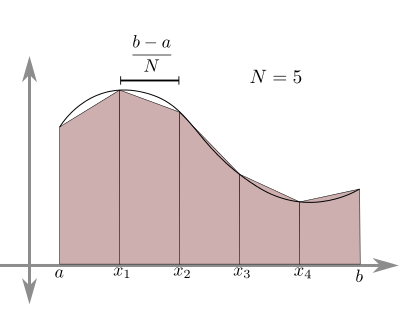
\includegraphics[width=.5\textwidth]{trapezoid_rule_theory_placeholder.png}
\caption{The trapezoid rule in action. TODO get a copyright-kosher version.}
\label{fig:trapezoid_rule}
\end{figure}
% I took this template for including images from the data structures lab

The following Python program is a simple serial (as opposed of parallel)
implementation of the trapezoid rule:

\lstinputlisting[style=fromfile]{trapSerial.py}

This serial implementation will be the basis for our parallel implementation.

\section*{Parallelizing the Trapezoid Rule}
\emph{The first and most important step in parallelizing an algorithm is
determining which steps of the algorithm can be computed independently}. In this
case, it is easy to see that the area of each trapezoid can be calculated
independently.

Currently, the algorithm divides up the interval $[a,b]$ into $n$ subintervals.
To parallelize this process, we will distribute these $n$ subintervals to the
available processes:

\lstinputlisting[style=fromfile, label=lst:MPI_Intro:trapParallel.py]{trapParallel.py}

In this parallel approach, the original interval is split such that each process
gets an equal-sized subinterval to integrate. After integrating, each process
sends its result to the root node, which sums up the values and displays the
final result. Although this is fairly straightforward, there are two important
things to note:

First, notice how the trapezoids are divided among the processes: The processors
each individually calculate what their \li{local_a}, \li{local_b}, and
\li{local_n} should be. We could have written the algorithm in a way such that
the root process figures out these values for every process and then tells each
process what their values should be. However, this would introduce an
unnecessary bottleneck: all of the other processes would be idling while waiting
for their assignment to arrive from the root process. By having each process
calculate its own range, we gain a large speedup. (Keep this in mind for problem
\ref{prob:MPI_Intro:trapParallelLoadBalanced.py})

Second, notice how the results are summed. We know how many results we should be
receiving, so the root process simply accepts the messages in the order that
they arrive. This is achieved using the tag \li{MPI.ANY_SOURCE} in the
\li{COMM.Recv} method, rather than insisting that the results arrive in order.
In lab \ref{lab:MPI_Collective_Communication}, we will learn about even more
effective ways to gather results from many different processes.
% todo link to lab where we learn gather (next lab). Talk about the speed up we
% gained here? but in this case there is no speedup...

We have successfully parallelized our first algorithm!

\section*{Load Balancing}
Although we have parallelized the trapezoid rule, our algorithm is still rather
naive. Notice that if the number of processes does not evenly divide the number
of trapezoids, the code will break down. Try running the trapezoid program with
n = 10000 and n = 10007 trapezoids:
\begin{lstlisting}[style=ShellInput]
$ mpirun -n 4 python trapParallel.py 0.0 1.0 10000
$ mpirun -n 4 python trapParallel.py 0.0 1.0 10007
\end{lstlisting}
This will produce the following:
\begin{lstlisting}[style=ShellOutput]
With 10000 trapezoids, our estimate of the integral of x^2 from 0.0 to 1.0 is:
    0.333333335
With 10007 trapezoids, our estimate of the integral of x^2 from 0.0 to 1.0 is:
    0.333033634715
\end{lstlisting}

We know that the estimate of the integral should improve as $n$ grows larger,
but this doesn't seem to be the case. This is because \li{local_n}, the number
of trapezoids that each processor calculates, must clearly be an integer. To
solve this problem, we could require that the user always choose a value of $n$
that is divisible by the number of processors. However, \emph{good parallel
algorithms should let the user worry as little as possible about how the
parallelization works.} Good parallel algorithms' interfaces should generally be
almost exactly the same as a serial algorithm that gets the same result. Thus,
we should make our code more robust and make it work even if $n$ is not
divisible by the number of processes.

One way to solve this problem would be to designate one process to handle the
leftover trapezoids that; i.e. give each process \li{int(n/SIZE)} trapezoids and
assign an additional \li{n \% SIZE} trapezoids to the last process. Thus, the
\li{local_n} of each process would be an integer. However, this method can be
incredibly inefficient; suppose we ran the program with 100 processes and 1099
trapezoids? Then each process would have \li{int(1099/100) = 10} trapezoids to
calculate... except for the last process, which would have \li{int(1099/100)
+ (1099 \% 100) = 109} trapezoids!

\emph{A parallel program can only be as fast as its slowest process.} We call
this principle \emph{load balancing}. In this case, one process has to do over
ten times as much work as the other processes! The other processes will end up
waiting idle until the last one finishes. Ignoring communication costs and other
overhead, this program could be nearly \emph{10 times faster} if we divided up the work
more evenly!

In the case of the trapezoid rule, load-balancing the code means two things.
First, for any two processes, the number of trapezoids assigned to each process
should differ by at most 1. Second, each process should estimate the area of a
contiguous group of trapezoids. Although estimating an integral is not a very
time-consuming operation, by estimating over contiguous groups of trapezoids we
are minimizing the amount of duplicate work the processes have to do, which is
good practice.

\begin{problem}
Implement the load-balancing fix to the code \texttt{trapParallel.py}. The
program should be able to take in any number of trapezoids $n$ for any number of
processes and the trapezoids should be divided among the processes evenly,
differing by at most one between any two processes. Each process should
independently calculate which section of trapezoids it should calculate.

For example, if the program is run with 5 processes and 12 trapezoids, processes
0 should calculate the first 3 trapezoids, process 1 should calculate the next 3
trapezoids, process 2 should calculate the next 2 trapezoids, process 3 should
calculate the next 2 trapezoids, and process 4 should calculate the last 2
trapezoids.
\label{prob:MPI_Intro:trapParallelLoadBalanced.py}
\end{problem}

\section*{Speed}

TODO

Talk about how we reduced function calls by 2x from original equation
Talk about how parallel speedup is limited, especially in this case. (Also in general due to how \emph{expensive} communication is)
